\documentclass[11pt,a4paper]{article}
\author{TalentSprint}
\date{}
\usepackage{graphicx}
\usepackage{verbatim}
\usepackage{array}
\usepackage{caption}
\usepackage{enumitem}
\usepackage{xcolor}
\usepackage[tikz]{bclogo}
\usepackage{textcomp}
\usepackage{listings}
\usepackage{multicol}
\usepackage{float}
\usepackage{seqsplit} 
\usepackage{setspace}
\usepackage{soul}
\usepackage{latexsym}
\lstset{language=Java,numbers=left, numberstyle=\tiny, numbersep=10pt, showstringspaces=false, breaklines=true,keepspaces=true, columns=flexible}
\usepackage{fancyhdr}
\headheight=14pt
\lhead{\nouppercase{}}
\rhead{\nouppercase{\leftmark}}

\graphicspath{{../Images/}}


\begin{comment}
\setcounter{tocdepth}{1}
\setlength\parindent{0pt}
\parskip=4pt
\def\AnswerBox{\fbox{\begin{minipage}{4in}\hfill\vspace{0.5in}\end {minipage}}}

\thispagestyle{empty}
\vspace{1.5pc}
\topskip0pt
\vspace*{\fill}
\centerline{\sc \Huge Version Control System}
\vspace{2pc}
\vspace*{\fill}
\centerline{Prepared by TalentSprint WISE Team} 
\setcounter{page}{1}
\pagestyle{fancy}
\end{comment}


%========================================================================

% Lengths and widths
\addtolength{\textwidth}{2.5cm}
\addtolength{\hoffset}{0cm}
\setlength{\headsep}{-12pt} % Reduce space between header and content
\setlength{\headheight}{85pt} % If less, LaTeX automatically increases it
\renewcommand{\footrulewidth}{2pt} % Remove footer line
\renewcommand{\headrulewidth}{1pt} % Remove header line
\renewcommand{\seqinsert}{\ifmmode\allowbreak\else\-\fi} % Hyphens in seqsplit
% This two commands together give roughly
% the right line height in the tables
\renewcommand{\arraystretch}{1.3}
\onehalfspacing



% Commands
\newcommand{\SetRowColor}[1]{\noalign{\gdef\RowColorName{#1}}\rowcolor{\RowColorName}} % Shortcut for row colour
\newcommand{\mymulticolumn}[3]{\multicolumn{#1}{>{\columncolor{white}}#2}{#3}} % For coloured multi-cols
\newcolumntype{x}[1]{>{\raggedright}p{#1}} % New column types for ragged-right paragraph columns
\newcommand{\tn}{\tabularnewline} % Required as custom column type in use

% Font and Colours
\definecolor{HeadBackground}{HTML}{333333}
\definecolor{FootBackground}{HTML}{666666}
\definecolor{TextColor}{HTML}{333333}
\definecolor{DarkBackground}{HTML}{6B8E23} %{FD1AA8}
\definecolor{LightBackground}{HTML}{E8FED8} %D3FDC8
\definecolor{tit}{HTML}{FF6600}
\renewcommand{\familydefault}{\sfdefault}
\color{TextColor}
 \headsep = 25pt
% Header and Footer
\pagestyle{fancy}
\usepackage[headheight=110pt]{geometry}
\fancyhf{}% Clear header/footer

\fancyhead[r]{
\includegraphics[width = 4cm, height = 2cm]{TS-Logo.png}\hspace{0cm}}

%=================================TITLE=====================================
\fancyhead[l]{{\bf{\textcolor{tit}{\textrm{\large{Inheritance and Polymorphism}}}}}}
%===========================================================================

\renewcommand{\headrulewidth}{0.4pt}% Default \headrulewidth is 0.4pt
\renewcommand{\footrulewidth}{0.4pt}% Default \footrulewidth is 0pt

\rfoot{Page \thepage}
\lfoot{COPYRIGHT \textcopyright TALENTSPRINT, 2015. ALL RIGHTS RESERVED.}


\begin{document}
\section*{Inheritance}
 In real life you can observe inheritance almost everywhere. A child for example takes on the characteristics of parents. It is so in OOP also.
 This is one of the most powerful feature of OOP.
 
\emph{\textbf{Inheritance}} is the concept of a child class (subclass) automatically inheriting the variables and methods defined in its parent class (superclass). It is the mechanism through which a class can be defined in terms of an existing class.
 
 \begin{figure}[H] 
 \begin{center}
   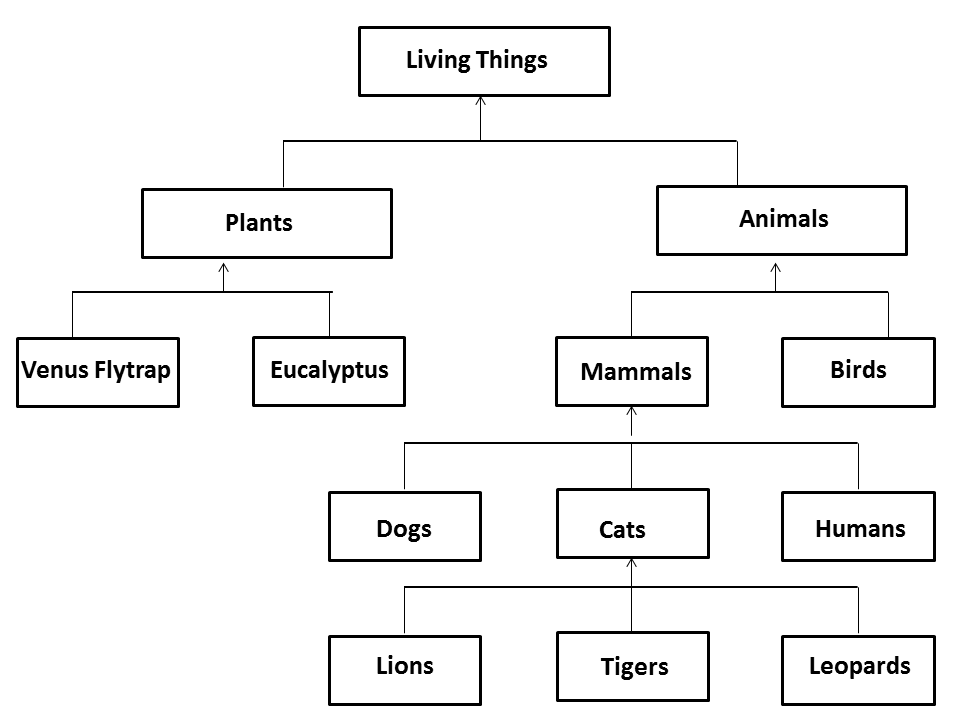
\includegraphics[scale=.35]{Inheritance.png}
   \caption{Inheritance Example}
 \end{center}
 \end{figure}
 
Inheritance enables the refinement or specialization of an existing class. Through inheritance a child can acquire characteristics of its parents and can also have its own features.
 
 In the above diagram plant `Venus Flytrap' not only inherits the characteristics of plants and also has features by which it traps and eats insects.

 \subsection*{Importance of inheritance}
 \begin{itemize}
  \item The benefit of inheritance in OOP is reusability. Once a behavior (method) is defined in a superclass, that behavior is automatically inherited by all subclasses.
  \item Once a set of properties (fields) are defined in a superclass, the same set of properties are inherited by all subclasses. A class and its children share common set of properties.
  \item A subclass only needs to implement the differences between itself and the parent.

 \end{itemize}

 The class that inherits a set of attributes is called as \textbf{subclass} or \textbf{derived class} and the class from which it inherits is called as \textbf{superclass} or \textbf{parent class}. We can define inheritance is an OOP term, in which the non-private features and attributes of a given superclass are made available to its subclass(es).
 
 A subclass acquires the properties from superclass using a keyword \emph{\textbf{extends}}. 
 
 \subsection*{Deriving a subclass}
\begin{itemize}
\item To derive a child class, you use the \lstinline!extends! keyword.
\item Suppose you have a parent class called Person.
 
%  \textbf{Defining super / parent class}
 \lstinputlisting{../Code/Person.java}
 
  \item Now, create another class named Student.
  \item Since a student is also a person, just extend the class `Person', so that `Student' class can inherit all the properties and methods of the existing class Person.
  \item To do this, use \emph{extends} keyword and write as below,
  
  \lstinputlisting{../Code/Student.java}
\end{itemize}
%=====================================================================================================================================
 
 Inheritance defines \textbf{is a} relationship between the classes.
 
 \begin{figure}[H] 
 \begin{center}
  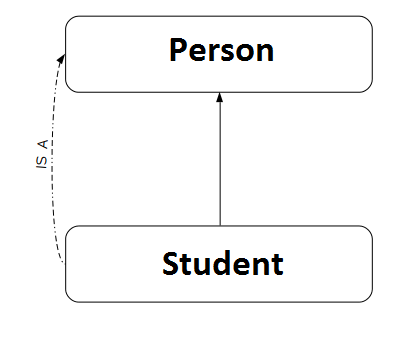
\includegraphics[scale=.5]{is_a_Relation.png}
   \caption{Single Inheritance}
 \end{center}
 \end{figure}
 
 From the above example, we can say \emph{Student} \textbf{is a} \emph{Person}.
 \subsubsection*{What a subclass can do}
 \begin{itemize}
  \item  A subclass inherits all of the “public” and “protected” members (fields or methods) of
its parent, no matter what package the subclass is in.
  \item If the subclass is in the same package as its parent, then it also inherits the package-
private members (fields or methods) of the parent.

 \end{itemize}
 
\subsubsection*{What a sub-class can do regarding fields}
\begin{itemize}
\item The inherited fields can be used directly, just like any other fields.
\item Can declare new fields in the subclass that are not in the superclass.
\item Can declare a field in the subclass with the same name as the one in the superclass, thus hiding it (not recommended).
\item A subclass does not inherit the private members of its parent class. However, if the superclass has public or protected methods for accessing its private fields, these can also be applied by the subclass.
\end{itemize}

\subsubsection*{What a subclass can do regarding methods}
\begin{itemize}
\item The inherited methods can be used directly as they are.
\item Can write a new instance method in the subclass that has the same signature as the one in the superclass, thus overriding it.
\item Can write a new static method in the subclass that has the same signature as the one in the superclass, thus hiding it.
\item Can declare new methods in the subclass that are not in the superclass.
\end{itemize}

\section*{Types of inheritance}
Java can implement inheritance in the following types.
 
\begin{description}
\item[Single/Simple Inheritance]\
  
Single inheritance enables a derived class to inherit properties and behavior from a single base class.
     
 \begin{figure}[H] 
 \begin{center}
 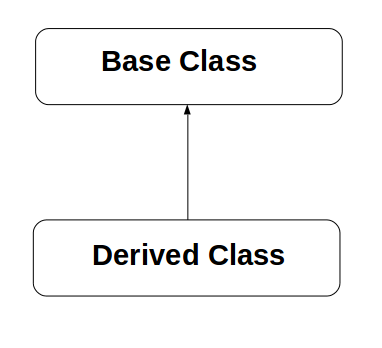
\includegraphics[scale=.5]{single_inheritance.png}
   \caption{Single Inheritance}
 \end{center}
 \end{figure}
 
As it allows a derived class to inherit the properties and behavior of a base class, thus enabling code reusability as well as adding new features to the existing code. This makes the code much more elegant and less repetitive. 
\item[Multilevel Inheritance]\
  
Multilevel inheritance enables a derived class to inherit properties and behavior from another derived class, which is inherited from a base class.
   
\begin{figure}[H] 
\begin{center}
   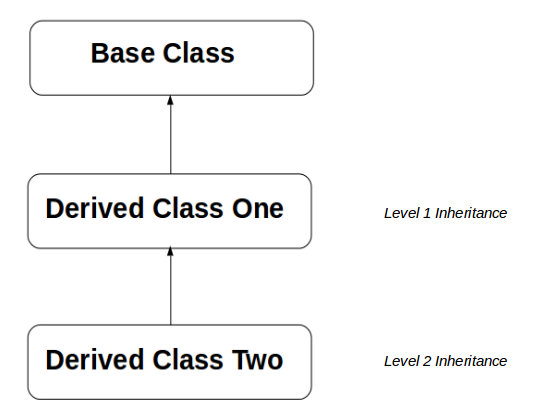
\includegraphics[scale=.35]{multilevel_inheritance.png}
   \caption{Multilevel Inheritance}
\end{center}
\end{figure}
 
In this process inheritance builds different levels, thats why this type of inheritance is called as \emph{multilevel inheritance}.
 
 % \lstinputlisting[firstline=6, lastline=20]{../Code/MultilevelInheritance.java}
 
 \item[Hierarchical Inheritance]\
 
 Hierarchical inheritance enables a base class to inherit its properties and behavior to multiple derived classes.
 
\begin{figure}[H] 
\begin{center}
  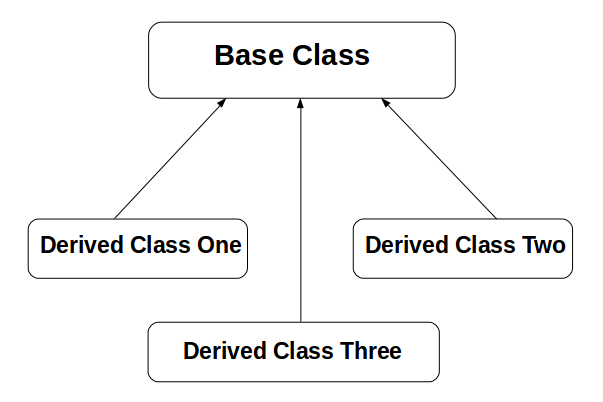
\includegraphics[scale=.35]{hierarchical_inheritance.png}
   \caption{Hierarchical Inheritance Example}
\end{center}
\end{figure}
 
 \end{description}
 
  \begin{figure}[H]
 \begin{center}
   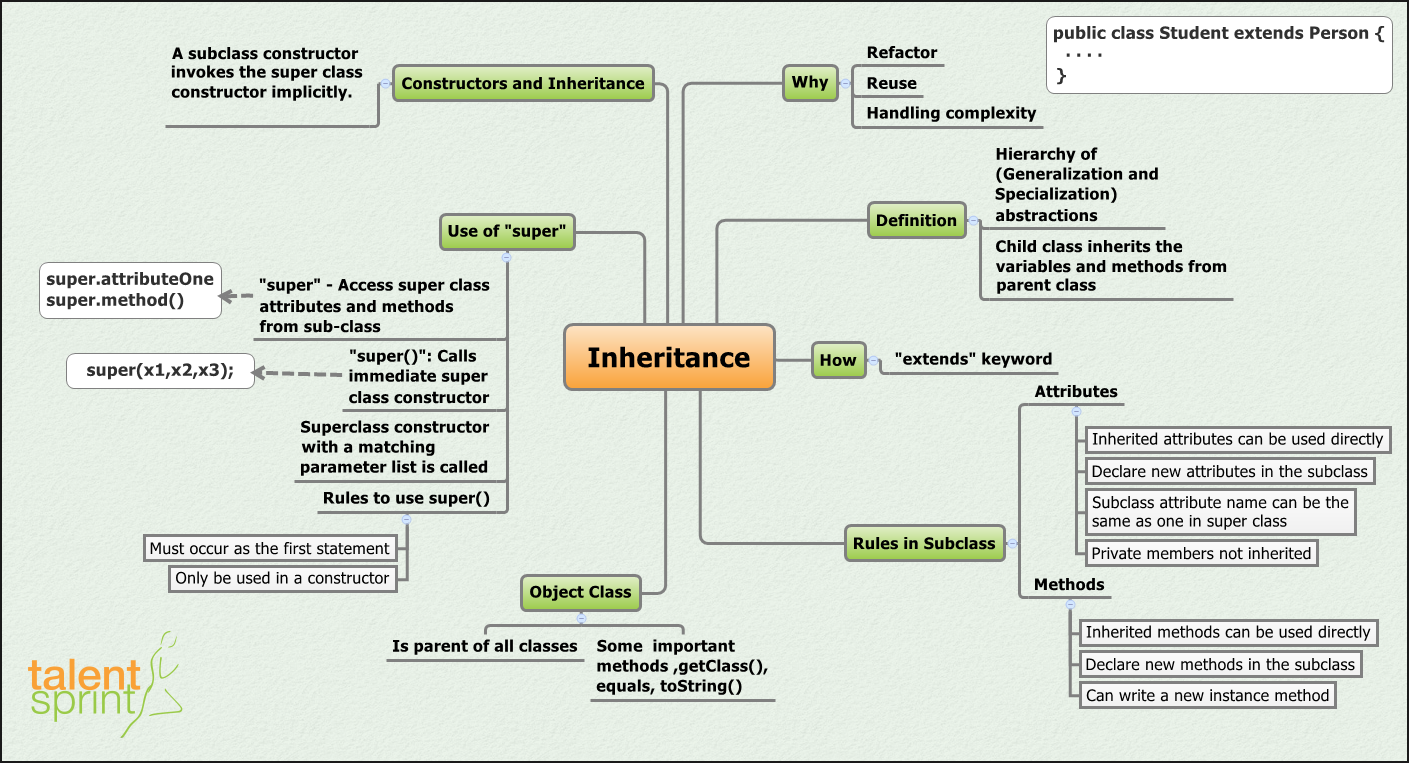
\includegraphics[angle=90,height=20cm, width=13cm]{Inheritance-MM.png}
  
 \end{center}
 \end{figure}
 
 \section*{`super' keyword}
In base class members are overriden by its derived class, hence base class members are hidden on accessing.

To refer the overriden members of base class, in Java \emph{\textbf{super}} keyword is used.
 
 Assume the below class is base class.
 \lstinputlisting{../Code/BaseClass.java}
  
 \begin{description}
  \item Compile the above program
  \begin{verbatim}
  $ javac BaseClass.java
 \end{verbatim}
 \textbf{Example without using super} 
 
 \lstinputlisting{../Code/WithOutSuperDemo.java}
 \begin{figure}[H] 
 \begin{center}
   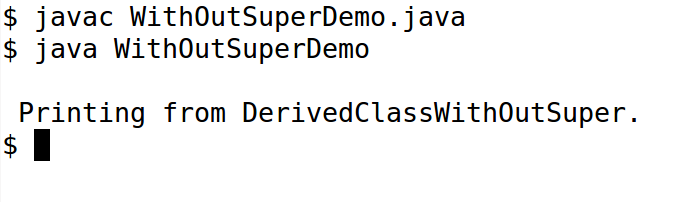
\includegraphics[scale=.4]{WithOutSuperDemo.png}
   \caption*{Output: WithOut Super}
 \end{center}
 \end{figure}
 \textbf{Example using super} 
 \lstinputlisting{../Code/WithSuperDemo.java}
 \begin{figure}[H] 
 \begin{center}
   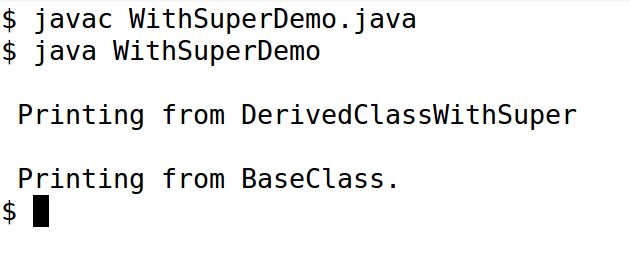
\includegraphics[scale=.4]{WithSuperDemo.png}
   \caption*{Output: With Super}
 \end{center}
 \end{figure}
 

super as a base class constructor
 
 \lstinline!super! keyword is also used to invoke base class constructor from derived class.\\
 
 \textbf{Example for super used as a constructor.} \\
 \textbf{superclass definition}
 
 \lstinputlisting{../Code/SuperClass.java}
 \textbf{derived class definition}
 \lstinputlisting{../Code/SuperConstructor.java}
 
 \begin{figure}[H] 
 \begin{center}
   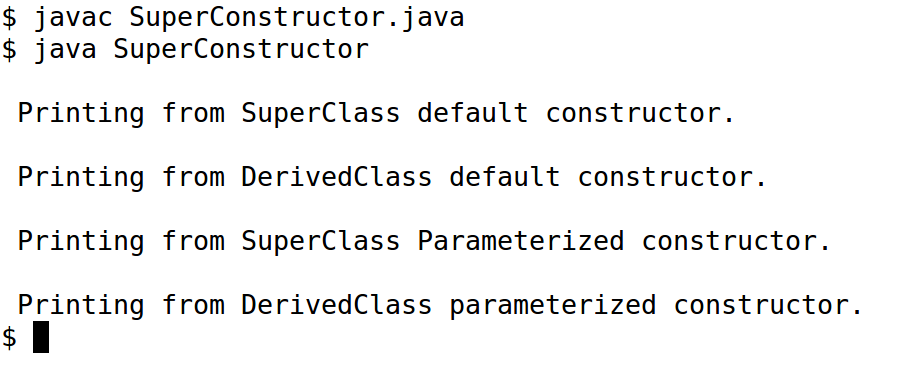
\includegraphics[scale=.4]{SuperConstructor.png}
   \caption*{Output: SuperConstructor}
 \end{center}
 \end{figure}
\end{description}

\section*{Polymorphism}
The dictionary definition of \emph{\textbf{polymorphism}} refers to a principle in biology in which an organism or species can have many different forms or stages. This principle can also be applied to object-oriented programming.
 
 Java supports two types of polymorphism 
 \subsection*{Static Polymorphism} 
 In Java, static polymorphism is achieved through \emph{\textbf{method overloading}}.\\
 A Java class can define more than one methods with same name, that approach is called as \emph{\textbf{method overloading}} and also known as \emph{\textbf{Static / Compile-Time Polymorphism}}.
 
 \subsubsection*{Method overloading}
 
 \begin{itemize}
  \item Allows a method with the same name but different parameters, to have different implementations and return values of different types
  \item Can be applied when the same operation has different implementations
  \item Always remember that overloaded methods have the following properties:
  \begin{enumerate}
   \item The same method name
   \item Different parameters or different number of parameters
   \item Return types can be different or same
  \end{enumerate}

 \end{itemize}
 Assume a class `\emph{StudentRecord}' defines overloaded methods
  \lstinputlisting{../Code/StudentRecord.java}
  
  Set the values and run `\emph{StudentRecord}' class by creating instance.
  
  \lstinputlisting{../Code/StaticPolymorphismDemo.java}
 \begin{figure}[H] 
 \begin{center}
   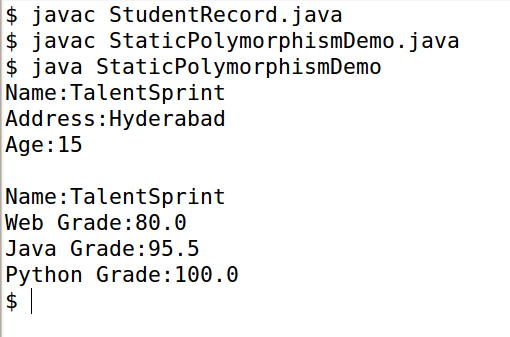
\includegraphics[scale=.5]{StaticPolymorphismDemo.png}
   %\caption*{\textbf{Output:} StaticPolymorphismDemo}
 \end{center}
 \end{figure}

 \subsection*{Dynamic Polymorphism} 
 In Java subclasses of a class can define their own unique behaviors and yet share some of the same functionality of the parent class.
 
 In Java, dynamic polymorphism is achieved through method overriding.
 
 Having the same method of base class in its derived class is called as \emph{\textbf{Method Overriding}}.

 Assume that `Animal' is a super class that contains a method `speak()'.
\lstinputlisting[firstline=1, lastline=6]{../Code/DynamicPoly.java}
 A derived class `Cat' inherits `Animal' class and overrides `speak()' method.
\lstinputlisting[firstline=7, lastline=12]{../Code/DynamicPoly.java}
The below code snippet shows how dynamic polymorphism works.
\lstinputlisting{../Code/DynamicPolymorphismDemo.java}
%\lstinputlisting[firstline=33, lastline=38]{../Code/DynamicPolymorphismDemo.java}
%\lstinputlisting[firstline=40, lastline=45]{../Code/DynamicPolymorphismDemo.java}

  \begin{figure}[H] 
 \begin{center}
   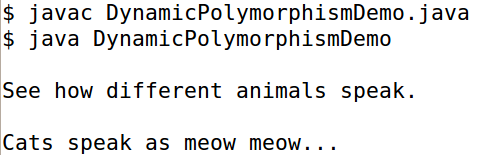
\includegraphics[scale=.5]{DynamicPolymorphismDemo.png}
   %\caption*{\textbf{Output:} DynamicPolymorphismDemo}
 \end{center}
 \end{figure}

 The above defined polymorphism is also known as \emph{\textbf{Dynamic/Runtime Polymorphism}}.

 Both the classes (Animal and Cat) have a common method \emph{speak()}.
\vfill{\ }
\subsubsection*{Difference between Overloading and Overriding}

\begin{table}[H]
\centering
\begin{tabular}{|p{5.5 cm}|p{5.5 cm}|} \hline

%\multicolumn{3}{|c|}{\textbf{Attributes}}\\\hline
\multicolumn{1}{|c|}{\textbf{Overloading} } & \multicolumn{1}{|c|}{\textbf{Overriding}} \\\hline
Signature has to be different. Just a difference in return type is not enough. & Signature has to be the same. (including the return type)\\\hline
Accessibility may vary freely. & Overriding methods cannot be more private than the overridden methods. \\ \hline
Just the name is reused. Methods are independent methods. Resolved at compile-time based on method signature. & Related directly to sub-classing. Overrides the parent class method. Resolved at run-time based on type of the object. \\ \hline
Can call each other by providing appropriate argument list. & Overriding method can call overridden method by super.methodName() , this can be used only to access the immediate method of superclass. super.super will not work. Also, a class outside the inheritance hierarchy cannot use this technique. \\ \hline
Methods can be static or non-static. If two methods have the same signature, declaring one as static and another as non-static does not provide a valid overload. It’s a compile time error. & static methods do not participate in overriding, since they are resolved at compile time based on the type of reference variable. A static method in a sub-class cannot use super. A static method cannot be overridden to be non-static and vice-versa. \\ \hline 
There is no limit on number of overloaded methods a class can have. & Each parent class method may be overridden at most once in any sub-class.\\ \hline

\end{tabular}
\end{table}
\vfill{\ }
\begin{figure}[H]
 \begin{center}
   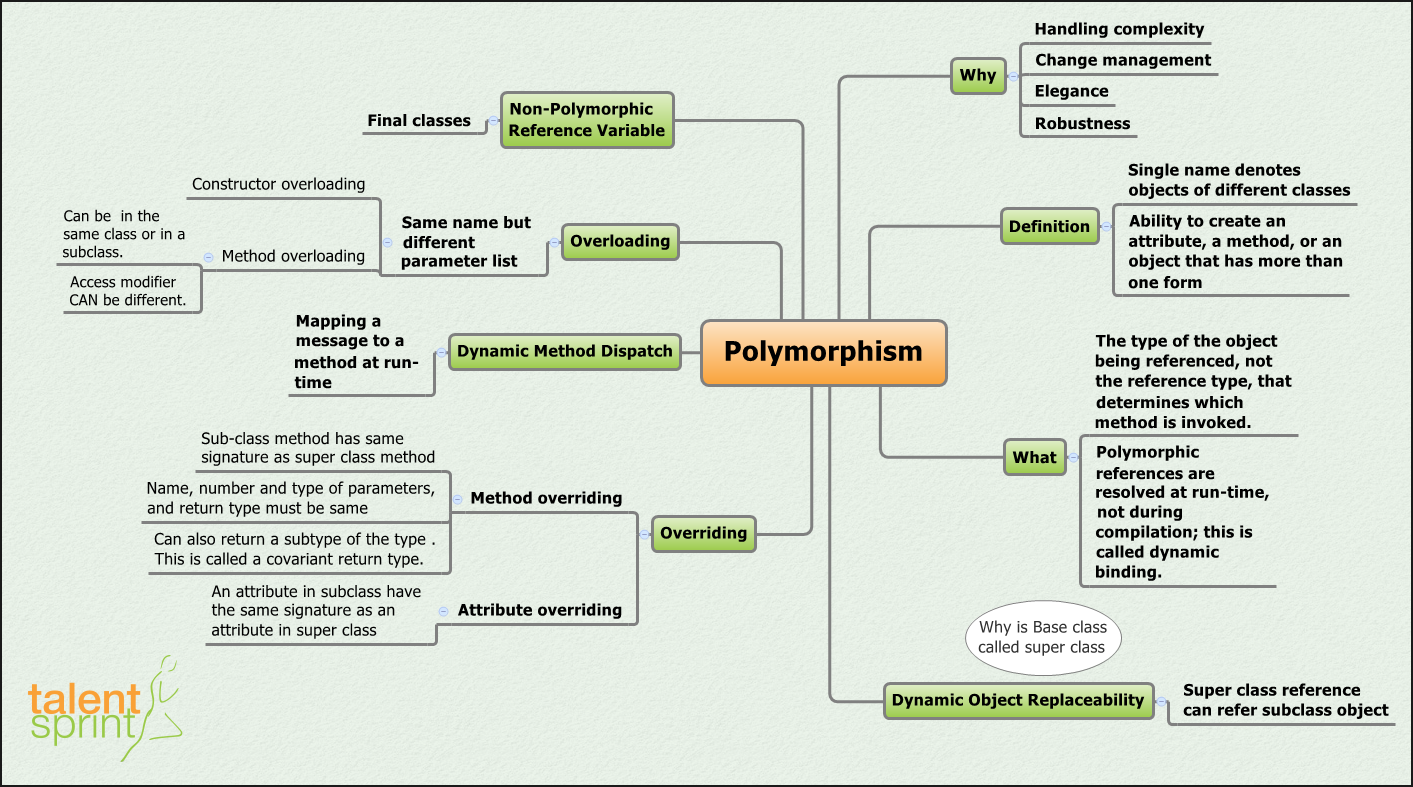
\includegraphics[angle=90,height=20cm, width=13cm]{Polymorphism.png}
  
 \end{center}
 \end{figure}




\end{document}